\part{Présentation de codes}

\section{Précautions}\label{codenumlignes}

\begin{tipblock}
L'idée est de proposer des environnements pour présenter du code :

\begin{itemize}
	\item \textsf{Python} ;
	\item \textsf{PseudoCode}.
\end{itemize}

Dans la mesure du possible (mis à part pour certains points avec l'utilisation des packages \ctex{piton} et \ctex{pythontex}), les environnements seront composés :

\begin{itemize}
	\item dans une boîte \ctex{tcolorbox} ;
	\item de deux styles : \ctex{CodeXXXX} ou \ctex{CodeXXXXAlt} ;
	\item de clés pour paramétrer la \Cle{Largeur} et le début de la numérotation \Cle{PremLigne} ;
	\item d'une version étoilée pour ne pas numérotée les lignes ;
	\item d'options éventuelles à donner en langage \ctex{tcolorbox}.
\end{itemize}
\vspace*{-\baselineskip}\leavevmode
\end{tipblock}

\begin{warningblock}
Avec la mise à jour \cmaj{2.7.5} et la possibilité de modifier la numérotation des lignes, certains environnements ont vu leur fonctionnement légèrement modifié, donc il est conseillé d'être prudent avec les nouvelles spécificités.

\smallskip

Il est prévu, à plus ou moyen terme, d'uniformiser le fonctionnement de tous les environnements, mais cela demande de reprendre une bonne partie du code.
\end{warningblock}

\section{Code Python \og simple \fg{} via le package listings}\label{pythonsimple}

\subsection{Introduction}

\begin{tipblock}
Le {package} \ctex{listings} permet d'insérer et de formater du code, notamment du code \textsf{Python}.

En \textit{partenariat} avec \ctex{tcolorbox}, on peut donc présenter \textit{joliment} du code \textsf{Python} !
\end{tipblock}

\begin{noteblock}
Le package \ctex{listings} ne nécessite pas de compilation particulière, au contraire d'autres (comme \ctex{pythontex} ou \ctex{\sout{minted}} ou \ctex{piton}) qui seront présentés ultérieurement.
\end{noteblock}

\begin{noteblock}
Les styles utilisés pour formater le code \textsf{Python} ne sont pas modifiables. Ils donnent un rendu proche de celui des packages comme \ctex{pythontex} ou \ctex{\sout{minted}} ou \ctex{piton}.

\smallskip

Donc, si plusieurs \textit{méthodes} sont utilisées pour insérer du code \textsf{Python} (via les \textit{méthodes} suivantes), le rendu pourra être légèrement différent.
\end{noteblock}

\subsection{Commande et options}

\begin{tipblock}
L'environnement \ctex{CodePythonLst} permet de présenter du code \textsf{Python}, dans une \ctex{tcolorbox} avec deux styles particuliers (\cmaj{2.5.8}).
\end{tipblock}

\begin{PresCodeTexPL}{listing only}
\begin{CodePythonLst}(*)[clés]{commandes tcbox}
...
\end{CodePythonLst}
\end{PresCodeTexPL}

\begin{PresCodeTexPL}{listing only}
\begin{CodePythonLstAlt}(*)[clés]{commandes tcbox}
...
\end{CodePythonLstAlt}
\end{PresCodeTexPL}

\begin{cautionblock}
Plusieurs \Cle{arguments} sont disponibles :

\begin{itemize}
	\item la version \textit{étoilée} qui permet de ne pas afficher les numéros de lignes ;
	\item le premier argument (\textit{optionnel}), comprend la clé \Cle{Largeur} de la \ctex{tcbox} (\Cle{\textbackslash linewidth} par défaut) et la clé \Cle{PremLigne} (\Cle{1} par défaut) et la clé \Cle{EspaceNum} (\Cle{14pt} par défaut) ;
	\item le second argument (\textit{obligatoire}), concerne des \Cle{options} de la \ctex{tcbox} en \textit{langage tcolorbox}, comme l'alignement.
\end{itemize}
\vspace*{-\baselineskip}\leavevmode
\end{cautionblock}

\begin{warningblock}
Les environnements créés par \ctex{tcolorbox} et \ctex{listings} ne sont pas compatibles avec les options \Cle{gobble} (pour supprimer les tabulations d'environnement), donc il faut bien penser à \og aligner \fg{} le code à gauche, pour éviter des tabulations non esthétiques !
\end{warningblock}

\subsection{Insertion via un fichier \og externe \fg}

\begin{tipblock}
Pour des raison pratiques, il est parfois intéressant d'avoir le code \textsf{Python} dans un fichier externe au ficher \ctex{tex}, ou bien créé directement par le fichier \ctex{tex} (via \ctex{scontents}, notamment, mais non chargé par \ctex{ProfLycee}).

Dans ce cas, il n'est pas nécessaire d'aligner le code \og à gauche \fg, en utilisant une commande alternative.

\smallskip

Si cette méthode est utilisée, il ne faut oublier de charger le package \ctex{scontents}, et être attentif à la syntaxe.
\end{tipblock}

\begin{PresCodeTexPL}{listing only}
\usepackage{scontents} %si script déclaré dans le fichier tex
...
\CodePythonLstFichier(*)[largeur]{commandes tcbox}{script}
\end{PresCodeTexPL}

\subsection{Exemples}

\begin{PresCodeTexPL}{listing only}
\begin{CodePythonLst}{} %les {}, même vides, peuvent être nécessaires (bug avec # sinon !)
#environnement par défaut
nb = int(input("Saisir un entier positif"))
if (nb %7 == 0) :
	print(f"{nb} est bien divisible par 7")
#endif

def f(x) :
	return x**2
\end{CodePythonLst}
\end{PresCodeTexPL}

\begin{PresCodeSortiePL}{text only}
\begin{CodePythonLst}{}
#environnement par défaut
nb = int(input("Saisir un entier positif"))
if (nb %7 == 0) :
	print(f"{nb} est bien divisible par 7")
#endif

def f(x) :
	return x**2
\end{CodePythonLst}
\end{PresCodeSortiePL}

\begin{PresCodeTexPL}{listing only}
\begin{CodePythonLst}[PremLigne=10]{}
nb = int(input("Saisir un entier positif"))
if (nb %7 == 0) :
	print(f"{nb} est bien divisible par 7")
#endif
\end{CodePythonLst}
\end{PresCodeTexPL}

\begin{PresCodeSortiePL}{text only}
\begin{CodePythonLst}[PremLigne=10]{}
nb = int(input("Saisir un entier positif"))
if (nb %7 == 0) :
	print(f"{nb} est bien divisible par 7")
#endif
\end{CodePythonLst}
\end{PresCodeSortiePL}

\begin{PresCodeTexPL}{listing only}
\begin{CodePythonLstAlt}*[Largeur=0.75\linewidth]{flush right}
#largeur de 75%, sans numéro, et aligné à droite
nb = int(input("Saisir un entier Python positif"))
if (nb %7 == 0) :
	print(f"{nb} est bien divisible par 7")
#endif

def f(x) :
	return x**2
\end{CodePythonLstAlt}
\end{PresCodeTexPL}

\begin{PresCodeSortiePL}{text only}
\begin{CodePythonLstAlt}*[Largeur=0.75\linewidth]{flush right}
#largeur de 50%, sans numéro, et aligné à droite
nb = int(input("Saisir un entier Python positif"))
if (nb %7 == 0) :
	print(f"{nb} est bien divisible par 7")
#endif

def f(x) :
	return x**2
\end{CodePythonLstAlt}
\end{PresCodeSortiePL}

\begin{PresCodeTexPL}{listing only}
\begin{scontents}[overwrite,write-out=testscript.py]
# Calcul de la factorielle en langage Python
def factorielle(x):
	if x < 2:
		return 1
	else:
		return x * factorielle(x-1)

# rapidité de tracé
import matplotlib.pyplot as plt
import time
def trace_parabole_tableaux():
	depart=time.clock()
	X = [] # Initialisation des listes
	Y = []
	a = -2
	h = 0.001
	while a<2:
		X.append(a) # Ajout des valeurs
		Y.append(a*a) # au "bout" de X et Y
		a = a+h
	# Tracé de l'ensemble du tableau de valeurs
	plt.plot(X,Y,".b")
	fin=time.clock()
	return "Temps : " + str(fin-depart) + " s."
\end{scontents}

%environnement centré, avec numéros, largeur 9cm
\CodePythonLstFichier[9cm]{center}{testscript.py}
\end{PresCodeTexPL}

\begin{PresCodeSortiePL}{text only}
\begin{scontents}[overwrite,write-out=testscript.py]
# Calcul de la factorielle en langage Python
def factorielle(x):
	if x < 2:
		return 1
	else:
		return x * factorielle(x-1)

# rapidité de tracé
import matplotlib.pyplot as plt
import time
def trace_parabole_tableaux():
	depart=time.clock()
	X = [] # Initialisation des listes
	Y = []
	a = -2
	h = 0.001
	while a<2:
		X.append(a) # Ajout des valeurs
		Y.append(a*a) # au "bout" de X et Y
		a = a+h
	# Tracé de l'ensemble du tableau de valeurs
	plt.plot(X,Y,".b")
	fin=time.clock()
	return "Temps : " + str(fin-depart) + " s."
\end{scontents}

\CodePythonLstFichier[9cm]{center}{testscript.py}
\end{PresCodeSortiePL}

\newpage

\section{Code Python via le package piton}\label{pythonpiton}

\subsection{Introduction}

\begin{noteblock}
\cmaj{2.5.0} Cette section nécessite de charger la \textsf{librairie} \clib{piton} dans le préambule.

\cmaj{2.5.7} Une console \textsf{Python} est disponible, elle nécessite le package \ctex{pyluatex}, qui n'est pas chargé par \ctex{ProfLycee}, du fait de l'obligation de spécifier le \textit{chemin} pour l'exécutable \textsf{Python} !
\end{noteblock}

\begin{PresCodeTexPL}{listing only}
\usepackage[executable=...]{pyluatex} %si utilisation de la console REPL
\useproflyclib{piton}
\end{PresCodeTexPL}

\begin{noteblock}
La \textsf{librairie} \clib{piton} (qui charge \ctex{piton}, est compatible uniquement avec \hologo{LuaLaTeX} !) permet d'insérer du code \textsf{Python} avec une coloration syntaxique en utilisant la bibliothèque \textsf{Lua LPEG}.

\smallskip

En \textit{partenariat} avec \ctex{tcolorbox}, on peut avoir une présentation de code \textsf{Python} !

\smallskip

\cmaj{3.03c} Les options pour \Cle{gobble} sont disponibles et \textbf{à adapter en fonction des situations} (voir la doc de \textsf{piton}).

\smallskip

\cmaj{3.04d} Afin de faciliter l'écriture de codes, et de s'affranchir de l'aspect \textit{tabulation}, il est possible d'utiliser des \textbf{commandes} (avec les mêmes clés que les environnements) qui vont insérer le code inclus dans un fichier existant (ou créé avec \ctex{filecontents/scontents}).
\end{noteblock}

\begin{warningblock}
Le package \ctex{piton} nécessite donc obligatoirement l’emploi de \hologo{LuaLaTeX} !

Ce package n'est chargé que si la compilation détectée est en \hologo{LuaLaTeX} !

\smallskip

\cmaj{2.5.7} L'utilisation de la console \textbf{REPL} nécessite une compilation en \ctex{--shell-escape} ou \ctex{-write18} !

\cmaj{2.5.7} Les packages \ctex{pyluatex} et \ctex{pythontex} utilisent des commandes de même nom, donc la présente documentation n'utilisera pas le package \ctex{pyluatex}. Une documentation annexe spécifique est disponible.
\end{warningblock}

\subsection{Présentation de code Python}

\begin{PresCodeTexPL}{listing only}
\begin{CodePiton}[clés]{options tcbox}<option line-numbers>
...
\end{CodePiton}

%ou

\CodePitonFichier[clés]{fichier}<option line-numbers>
\end{PresCodeTexPL}

\begin{cautionblock}
Plusieurs \Cle{clés} sont disponibles :

\begin{itemize}
	\item la clé booléenne \Cle{Lignes} pour afficher ou non les numéros de lignes ; \hfill{}défaut \Cle{true}
	\item \cmaj{3.03c} la clé \Cle{Gobble} pour spécifier des options liées au \textsf{gobble}, parmi \Cle{nb/auto/...}, et \textbf{à adapter en fonction des situations} ;
	
	\hfill{}défaut \Cle{vide}
	\item la clé \Cle{Largeur} qui correspond à la largeur de la \ctex{tcbox} ; \hfill{}défaut \Cle{\textbackslash linewidth}
	\item la clé \Cle{TaillePolice} pour la taille des caractères ; \hfill{}défaut \Cle{\textbackslash footnotesize}
	\item la clé \Cle{Alignement} qui paramètre l'alignement de la \ctex{tcbox} ;  \hfill{}défaut \Cle{center}
	\item \cmaj{3.11e} la clé \Cle{Style} (parmi \Cle{Moderne / Classique / Onglet / Carbon / CarbonClair}) pour changer le style ;
	
	\hfill{}défaut \Cle{Classique}
	\item \cmaj{2.5.7} le boolén \Cle{Filigrane} pour afficher, le logo {\small \faPython} en filigrane ; \hfill{}défaut \Cle{false}
	\item \cmaj{2.5.7} le boolén \Cle{BarreTitre} (si \Cle{Style=Moderne}) pour afficher le titre ; \hfill{}défaut \Cle{true}
	\item \cmaj{2.5.7} le boolén \Cle{Cadre} (si \Cle{Style=Moderne}) pour afficher le cadre ; \hfill{}défaut \Cle{true}
	\item \cmaj{3.04f} la clé \Cle{CouleurNombres} pour la couleur des nombres ; \hfill{}défaut \Cle{orange!75!black}
	\item \cmaj{3.11e} la clé \Cle{Couleur} pour la couleur du style \Cle{Onglet} ; \hfill{}défaut \Cle{red}
	\item \cmaj{3.11e} la clé \Cle{IconesCarbon} pour les icônes des styles \Cle{Carbon*}.
\end{itemize}
\vspace*{-\baselineskip}\leavevmode
\end{cautionblock}

\begin{noteblock}
Du fait du paramétrage des boîtes \ctex{tcolorbox}, il se peut que le rendu soit non conforme si elle doit être insérée dans une autre \ctex{tcolorbox}\ldots{} (normalement corrigé en \cmaj{2.6.9}) !

\smallskip

La visualisation des différents styles est davantage présentée dans le document \texttt{ProfLycee-exemples-pyluatex.pdf}.
\end{noteblock}

\begin{warningblock}
Même si les options \textsf{Gobble} sont disponibles, la version \textit{par défaut} donne des résultats satisfaisants, à condition d'aligner le code au même niveau que le \verb*|\begin{...}...\end{...}|.
\end{warningblock}

\begin{noteblock}
Pour éviter des problèmes avec le code interprété par \textsf{piton}, les \ctex{\{\}} de l'argument obligatoire sont nécessaires au bon fonctionnement du code.
\end{noteblock}

\begin{PresCodeTexPL}{listing only}
\begin{CodePiton}{} %pour éviter un bug avec le caractère #
#environnement piton avec numéros de ligne, pleine largeur, style moderne
def arctan(x,n=10):
	if x < 0:
		return -arctan(-x) #> (appel récursif)
	elif x > 1:
		return pi/2 - arctan(1/x) #> (autre appel récursif)
	else:
		return sum( (-1)**k/(2*k+1)*x**(2*k+1) for k in range(n) )
\end{CodePiton}
\end{PresCodeTexPL}

\begin{CodePiton}{}
#environnement piton avec numéros de ligne, pleine largeur, style classique
def arctan(x,n=10):
	if x < 0:
		return -arctan(-x) #> (appel récursif)
	elif x > 1:
		return pi/2 - arctan(1/x) #> (autre appel récursif)
	else:
		return sum( (-1)**k/(2*k+1)*x**(2*k+1) for k in range(n) )
\end{CodePiton}

\begin{PresCodeTexPL}{listing only}
\begin{CodePiton}[Style=Moderne,Filigrane]{}<start=10>
#environnement piton avec numéros (début=10), style moderne, filigrane
def arctan(x,n=10):
	if x < 0:
		return -arctan(-x) #> (appel récursif)
	elif x > 1:
		return pi/2 - arctan(1/x) #> (autre appel récursif)
	else:
		return sum( (-1)**k/(2*k+1)*x**(2*k+1) for k in range(n) )
\end{CodePiton}
\end{PresCodeTexPL}

\begin{CodePiton}[Style=Moderne,Filigrane]{}<start=10>
#environnement piton avec numéros, style moderne, filigrane
def arctan(x,n=10):
	if x < 0:
		return -arctan(-x) #> (appel récursif)
	elif x > 1:
		return pi/2 - arctan(1/x) #> (autre appel récursif)
	else:
		return sum( (-1)**k/(2*k+1)*x**(2*k+1) for k in range(n) )
\end{CodePiton}

\begin{PresCodeTexPL}{listing only}
\begin{CodePiton}[Alignement=flush right,Largeur=13cm]{}
def f(x) :
	return x**2
\end{CodePiton}

\begin{CodePiton}[Alignement=flush left,Largeur=11cm]{}
def f(x) :
	return x**2
\end{CodePiton}

\begin{itemize} %Avec des indentations d'environnement :
	\item On essaye avec un \texttt{itemize} :
	%
	\begin{CodePiton}[Gobble=tabs,Largeur=12cm,Style=Classique,Cadre=false]{}
	def f(x) :
		return x**2
	\end{CodePiton}
	\item Et avec un autre \texttt{itemize} :
	%
	\begin{CodePiton}[Gobble=tabs,Largeur=12cm,Style=Moderne,Cadre=false,BarreTitre=false]{}
	#avec numéros, de largeur 12cm, centré, moderne, sans cadre/titre
	def f(x) :
		return x**2
	\end{CodePiton}
\end{itemize}
\vspace*{-\baselineskip}\leavevmode
\end{PresCodeTexPL}

\begin{CodePiton}[Alignement=flush right,Largeur=13cm]{}
#avec numéros, de largeur 13cm, aligné à droite
def f(x) :
	return x**2
\end{CodePiton}

\begin{CodePiton}[Alignement=flush left,Largeur=11cm]{}
#avec numéros, de largeur 11cm, aligné à gauche
def f(x) :
	return x**2
\end{CodePiton}

\begin{itemize}
	\item On essaye avec un \texttt{itemize} :
	%
	\begin{CodePiton}[Gobble=tabs,Largeur=12cm,Cadre=false]{}
	#avec numéros, de largeur 12cm, centré, classique, sans cadre
	def f(x) :
		return x**2
	\end{CodePiton}
	\item Et avec un autre \texttt{itemize} :
	%
	\begin{CodePiton}[Gobble=tabs,Largeur=12cm,Style=Moderne,BarreTitre=false,Cadre=false]{}
	#avec numéros, de largeur 12cm, centré, moderne, sans cadre/titre
	def f(x) :
		return x**2
	\end{CodePiton}
\end{itemize}

\subsection{Console en partenariat avec Pyluatex}

\begin{noteblock}
\cmaj{2.5.7} Une console d'exécution (type REPL) est disponible, et la documentation associée est en marge de la présente documentation.
\end{noteblock}

\pagebreak

\section{Code \& Console Python, via le package Pythontex}

\subsection{Librairies}

\begin{noteblock}
\cmaj{2.5.0} Cette section nécessite de charger les librairies \ctex{\sout{minted}} ou \clib{pythontex} dans le préambule.

\smallskip

\cmaj{3.05b} {\small\faBomb} Suite à la mise à jour de \ctex{minted} en version 3.0, et en attendant une compatibilité de \ctex{tcblisting}, la librairie \clib{minted} est en \textit{standby}.
\end{noteblock}

\begin{PresCodeTexPL}{listing only}
%\useproflyclib{minted}
\useproflyclib{pythontex}
%ou
%\useproflyclib{minted,pythontex}
\end{PresCodeTexPL}

\subsection{Introduction}

\begin{tipblock}
\cmaj{2.5.0} La \textsf{librairie} \clib{pythontex} permet d'insérer et d'exécuter du code \textsf{Python}. On peut :

\begin{itemize}
	\item \cmaj{2.5.8} présenter du code \textsf{Python} (deux styles disponibles) ;
	\item exécuter du code \textsf{Python} dans un environnement type \og console \fg{} ;
	\item charger du code \textsf{Python}, et éventuellement l'utiliser dans la console.
\end{itemize}
\vspace*{-\baselineskip}\leavevmode
\end{tipblock}

\begin{warningblock}
\textbf{Attention : }il faut dans ce cas une compilation en plusieurs étapes, comme par exemple \textsf{pdflatex puis pythontex puis pdflatex} !

Voir par exemple \url{http://lesmathsduyeti.fr/fr/informatique/latex/pythontex/} !
\end{warningblock}

\begin{noteblock}
Compte tenu de la \textit{relative complexité} pour gérer les options (par paramètres/clés\ldots) des \textit{tcbox} et des \textit{fancyvrb}, les style sont \og fixés \fg{} tels quels, et seules la taille et la position de la \textit{tcbox} sont modifiables. Si toutefois vous souhaitez personnaliser davantage, il faudra prendre le code correspondant et appliquer vos modifications !

Cela peut donner -- en tout cas -- des idées de personnalisation en ayant une base \textit{pré}existante !
\end{noteblock}

\subsection{Présentation de code Python grâce au package pythontex}\label{pythontex}

\begin{tipblock}
L'environnement \ctex{CodePythontex} est donc lié à \ctex{pythontex} (chargé par \ctex{ProfLycee}, avec l'option \textit{autogobble}) permet de présenter du code \textsf{Python}, dans une \ctex{tcolorbox} avec deux styles particuliers (\cmaj{2.5.8}).
\end{tipblock}

\begin{PresCodeTexPL}{listing only}
\begin{CodePythontex}[clés]{} %les {} vides sont nécessaires
...
\end{CodePythontex}
\end{PresCodeTexPL}

\begin{PresCodeTexPL}{listing only}
\begin{CodePythontexAlt}[clés]{} %les {} vides sont nécessaires
	...
\end{CodePythontexAlt}
\end{PresCodeTexPL}

\begin{cautionblock}
Comme précédemment, des \Cle{Clés} qui permettent de \textit{légèrement} modifier le style :

\begin{itemize}
	\item \Cle{Largeur} : largeur de la \textit{tcbox} ;\hfill{}défaut \Cle{\textbackslash linewidth}
	\item \Cle{PremLigne} : numéro initial des lignes ; \hfill{}défaut \Cle{1}
	\item \Cle{TaillePolice} : taille des caractères ;\hfill{}défaut \Cle{\textbackslash footnotesize}
	\item \Cle{EspacementVertical} : option (\textit{stretch}) pour l'espacement entre les lignes ;\hfill{}défaut \Cle{1}
	\item \Cle{Lignes} : booléen pour afficher ou non les numéros de ligne.\hfill{}défaut \Cle{true}
\end{itemize}
\vspace*{-\baselineskip}\leavevmode
\end{cautionblock}

\begin{PresCodeTexPL}{listing only}
\begin{CodePythontex}{} %bien mettre les {} !!
	#environnement Python(tex) par défaut
	def f(x) :
		return x**2
\end{CodePythontex}
\end{PresCodeTexPL}

\begin{PresCodeSortiePL}{text only}
\begin{CodePythontex}{}
	#environnement Python(tex) par défaut
	def f(x) :
		return x**2
\end{CodePythontex}
\end{PresCodeSortiePL}

\begin{PresCodeTexPL}{listing only}
\begin{CodePythontexAlt}[Largeur=12cm,Centre,Lignes=false]{}
	#environnement Python(tex) classique, centré, sans lignes
	def f(x) :
		return x**2
\end{CodePythontexAlt}
\end{PresCodeTexPL}

\begin{PresCodeSortiePL}{text only}
\begin{CodePythontexAlt}[Largeur=12cm,Centre,Lignes=false]{}
	#environnement Python(tex) classique, centré, sans lignes
	def f(x) :
		return x**2
\end{CodePythontexAlt}
\end{PresCodeSortiePL}

%\subsection{Présentation de code Python via le package minted}\label{pytminted}
%
%\begin{noteblock}
%Pour celles et ceux qui ne sont pas à l'aise avec le {package} \ctex{pythontex} et notamment sa spécificité pour compiler, il existe le {package} \ctex{minted} qui permet de présenter du code, et notamment \textsf{Python}.
%
%\cmaj{2.5.8} Deux styles sont désormais disponibles.
%
%\cmaj{2.5.0} C'est donc la \textsf{librairie} \clib{minted} qu'il faudra charger.
%\end{noteblock}
%
%\begin{warningblock}
%Le package \ctex{minted} nécessite quand même une compilation avec l'option \ctex{--shell-escape} ou \ctex{-write18} !
%\end{warningblock}
%
%\begin{PresCodeTexPL}{listing only}
%\begin{CodePythonMinted}(*)[clés]{options tcbox}
%...
%\end{CodePythonMinted}
%\end{PresCodeTexPL}
%
%\begin{PresCodeTexPL}{listing only}
%\begin{CodePythonMintedAlt}(*)[clés]{options tcbox}
%...
%\end{CodePythonMintedAlt}
%\end{PresCodeTexPL}
%
%\begin{cautionblock}
%Plusieurs \Cle{arguments} sont disponibles :
%
%\begin{itemize}
%	\item la version \textit{étoilée} qui permet de ne pas afficher les numéros de lignes ;
%	\item le 1\up{er} argument (\textit{optionnel}), comprend la clé \Cle{Largeur} de la \ctex{tcbox} (\Cle{\textbackslash linewidth} par défaut) et la clé \Cle{PremLigne} (\Cle{1} par défaut) ;
%	\item le 2\up{nd} argument \textit{obligatoire} concerne les \Cle{options} de la \ctex{tcbox} en \textit{langage tcbox}.\hfill{}défaut \Cle{vide}
%\end{itemize}
%\vspace*{-\baselineskip}\leavevmode
%\end{cautionblock}
%
%\begin{PresCodeTexPL}{listing only}
%\begin{CodePythonMinted}[Largeur=13cm,PremLigne=10]{center}
%	#environnement Python(minted) centré avec numéros, de largeur 13cm
%	def f(x) :
%		return x**2
%\end{CodePythonMinted}
%\end{PresCodeTexPL}
%
%\begin{PresCodeSortiePL}{text only}
%\begin{CodePythonMinted}[Largeur=13cm,PremLigne=10]{center}
%	#environnement Python(minted) centré avec numéros
%	def f(x) :
%		return x**2
%\end{CodePythonMinted}
%\end{PresCodeSortiePL}
%
%\begin{PresCodeTexPL}{listing only}
%\begin{CodePythonMintedAlt}*[Largeur=0.8\linewidth]{}
%	#environnement Python(minted), style alt, sans numéro, de largeur 0.8\linewidth
%	def f(x) :
%		return x**2
%\end{CodePythonMintedAlt}
%\end{PresCodeTexPL}
%
%\begin{PresCodeSortiePL}{text only}
%\begin{CodePythonMintedAlt}*[Largeur=0.8\linewidth]{}
%	#environnement Python(minted), style alt, sans numéro, 0.8\linewidth
%	def f(x) :
%		return x**2
%\end{CodePythonMintedAlt}
%\end{PresCodeSortiePL}

\subsection{Console d'exécution Python}

\begin{tipblock}
\ctex{pythontex} permet également de \textit{simuler} (en exécutant également !) du code \textsf{Python} dans une \textit{console}, avec la \textsf{librairie} \clib{pythontex} du coup !

C'est l'environnement \ctex{ConsolePythontex} qui permet de le faire.
\end{tipblock}

\begin{PresCodeTexPL}{listing only}
\begin{ConsolePythontex}[clés]{} %les {} vides sont nécessaires
...
\end{ConsolePythontex}
\end{PresCodeTexPL}

\begin{cautionblock}
Les \Cle{Clés} disponibles sont :

\begin{itemize}
	\item \Cle{Largeur} : largeur de la \textit{console} ;\hfill{}défaut \Cle{\textbackslash linewidth}
	\item \Cle{Centre} : booléen pour centrer ou non la \textit{console} ;\hfill{}défaut \Cle{false}
	\item \Cle{TaillePolice} : taille des caractères ;\hfill{}défaut \Cle{\textbackslash footnotesize}
	\item \Cle{EspacementVertical} : option (\textit{stretch}) pour l'espacement entre les lignes ;\hfill{}défaut \Cle{1}
	\item \Cle{Label} : booléen pour afficher ou non le titre.\hfill{}défaut \Cle{true}
\end{itemize}
\vspace*{-\baselineskip}\leavevmode
\end{cautionblock}

\begin{PresCodeTexPL}{listing only}
\begin{ConsolePythontex}{}
	#console Python(tex) par défaut
	from math import sqrt
	1+1
	sqrt(12)
\end{ConsolePythontex}
\end{PresCodeTexPL}

\begin{PresCodeSortiePL}{text only}
\smallskip
\begin{ConsolePythontex}{}
	#console Python(tex) par défaut
	from math import sqrt
	1+1
	sqrt(12)
\end{ConsolePythontex}
\end{PresCodeSortiePL}

\begin{PresCodeTexPL}{listing only}
\begin{ConsolePythontex}[Largeur=14cm,Label=false,Centre]{}
	#console Python(tex) centrée sans label, 14cm
	table = [[1,2],[3,4]]
	table[0][0]
	
	from random import randint
	tableau = [[randint(1,20) for j in range(0,6)] for i in range(0,3)]
	tableau
	len(tableau), len(tableau[0]), tableau[1][4]
\end{ConsolePythontex}
\end{PresCodeTexPL}

\begin{PresCodeSortiePL}{text only}
\smallskip
\begin{ConsolePythontex}[Largeur=14cm,Label=false,Centre]{}
	#console Python(tex) centrée sans label, 14cm
	table = [[1,2],[3,4]]
	table[0][0]
	
	from random import randint
	tableau = [[randint(1,20) for j in range(0,6)] for i in range(0,3)]
	tableau
	len(tableau), len(tableau[0]), tableau[1][4]
\end{ConsolePythontex}
\end{PresCodeSortiePL}

\begin{noteblock}
Le package \ctex{pythontex} peut donc servir à présenter du code Python, comme \ctex{minted} ou \ctex{piton}, sa particularité est toutefois de pouvoir \textit{exécuter} du code \textsf{Python} pour une présentation de type \textit{console}.
\end{noteblock}

\newpage

\section{Pseudo-Code}\label{pseudocode}

\subsection{Introduction}

\begin{noteblock}
Le {package} \ctex{listings} permet d'insérer et de présenter du code, et avec \ctex{tcolorbox} on peut obtenir une présentation similaire à celle du code \textsf{Python}. Pour le moment la \textit{philosophie} de la commande est un peu différente de celle du code \textsf{Python}, avec son système de \Cle{Clés}.
\end{noteblock}

\subsection{Présentation de Pseudo-Code}

\begin{tipblock}
Les environnements \ctex{PseudoCode} ou \ctex{PseudoCodeAlt} permet de présenter du (pseudo-code) dans une \ctex{tcolorbox}, avec deux styles à disposition (\cmaj{2.5.8}).
\end{tipblock}

\begin{warningblock}
De plus, le package \ctex{listings} avec \ctex{tcolorbox} ne permet pas de gérer le paramètre \textit{autogobble}, donc il faudra être vigilant quant à la position du code (pas de tabulation en fait\ldots)
\end{warningblock}

\begin{PresCodeTexPL}{listing only}
\begin{PseudoCode}(*)[clés]{options tcbox}
%attention à l'indentation, gobble ne fonctionne pas...
...
\end{PseudoCode}
\end{PresCodeTexPL}

\begin{PresCodeTexPL}{listing only}
\begin{PseudoCodeAlt}(*)[clés]{options tcbox}
%attention à l'indentation, gobble ne fonctionne pas...
...
\end{PseudoCodeAlt}
\end{PresCodeTexPL}

\begin{cautionblock}
Plusieurs \Cle{arguments} (optionnels) sont disponibles :

\begin{itemize}
	\item la version \textit{étoilée} qui permet de ne pas afficher les numéros de lignes ;
	\item le 1\up{er} argument (\textit{optionnel}), comprend la clé \Cle{Largeur} de la \ctex{tcbox} (\Cle{\textbackslash linewidth} par défaut) et la clé \Cle{PremLigne} (\Cle{1} par défaut) et la clé \Cle{EspaceNum} (\Cle{14pt} par défaut) ;
	\item \cmaj{2.7.5} une clé booléenne \Cle{Couleur} est également disponible pour mettre en évidence trois niveaux (elles peuvent être redéfinies) de mots clés en pseudo-code (\Cle{false} par défaut) ;
	\item \cmaj{2.5.8} l'argument obligatoire entre \ctex{\{...\}} concerne les \Cle{options} de la \ctex{tcbox}.
\end{itemize}
\vspace*{-\baselineskip}\leavevmode
\end{cautionblock}

\begin{PresCodeTexPL}{listing only}
%en pas oublier les {}, même vides !
\begin{PseudoCode}{} %non centré, de largeur par défaut (12cm) avec lignes
List = [...]          # à déclarer au préalable
n = longueur(List)
Pour i allant de 0 à n-1 Faire
	Afficher(List[i])
FinPour
\end{PseudoCode}
\end{PresCodeTexPL}

\begin{PresCodeSortiePL}{text only}
\begin{PseudoCode}{}
List = [...]          # à déclarer au préalable
n = longueur(List)
Pour i allant de 0 à n-1 Faire
	Afficher(List[i])
FinPour
\end{PseudoCode}
\end{PresCodeSortiePL}

\begin{PresCodeTexPL}{listing only}
\begin{PseudoCodeAlt}[Largeur=15cm,PremLigne=7,Couleur]{center} %centré, de largeur 15cm
List = [...]          # à déclarer au préalable
n = longueur(List)
Pour i allant de 0 à n-1 Faire
	Afficher(List[i])
FinPour
\end{PseudoCodeAlt}
\end{PresCodeTexPL}

\begin{PresCodeSortiePL}{text only}
\begin{PseudoCodeAlt}[Largeur=15cm,PremLigne=7,Couleur]{center}
List = [...]          # à déclarer au préalable
n = longueur(List)
Pour i allant de 0 à n-1 Faire
	Afficher(List[i])
FinPour
\end{PseudoCodeAlt}
\end{PresCodeSortiePL}

\subsection{Compléments}

\begin{warningblock}
À l'instar de packages existants, la \textit{philosophie} ici est de laisser l'utilisateur gérer \textit{son} langage pseudo-code.

J'ai fait le choix de ne pas forcément définir des \textsf{mots clés} à mettre en valeur car cela reviendrait à \textit{imposer} des choix ! Donc ici, pas de coloration syntaxique (uniquement via la clé \Cle{Couleur}) ou de mise en évidence de mots clés, uniquement un formatage basique !
\end{warningblock}

\begin{PresCodeTexPL}{listing only}
%couleurs par défaut des mots clés, modifiables si besoin
\colorlet{MotsClesPseudoCodeA}{blue!75}
\colorlet{MotsClesPseudoCodeB}{green!50!black}
\colorlet{MotsClesPseudoCodeChaine}{red!75}
\end{PresCodeTexPL}

\begin{noteblock}
Le style \ctex{listings} utilisé par la commande a l'option \Cle{mathescape} activée, et accessible grâce aux délimiteurs \Cle{(*...*)}.

Cela permet d'insérer du code \LaTeX{} dans l'environnement \ctex{PseudoCode} (attention au fontes par contre !).
\end{noteblock}

\begin{PresCodeTexPL}{listing only}
\begin{PseudoCode}*[Largeur=12cm]{} % pour éviter un bug avec #
#Utilisation du mode mathescape
Afficher (*\og*) .........(*\fg*)
m = (*$\tfrac{\texttt{1}}{\texttt{2}}$*)
\end{PseudoCode}
\end{PresCodeTexPL}

\begin{PresCodeSortiePL}{text only}
\begin{PseudoCode}*[Largeur=12cm]{}
#Utilisation du mode mathescape
Afficher (*\og*) .........(*\fg*)
m = (*$\tfrac{\texttt{1}}{\texttt{2}}$*)
\end{PseudoCode}
\end{PresCodeSortiePL}

\newpage

\section{PseudoCode via le package piton}\label{pitonpcode}

\subsection{Introduction}

\begin{noteblock}
\cmaj{3.01f} Avec une version supérieure ou égale à \texttt{2.4} du package \ctex{piton}, il est possible d'utiliser un langage \texttt{minimal}, ce qui permet de pouvoir \textit{formater} du \textit{pseudocode}.

\smallskip

\cmaj{3.04d} Afin de faciliter l'écriture de codes, et de s'affranchir de l'aspect \textit{tabulation}, il est possible d'utiliser des \textbf{commandes} (avec les mêmes clés que les environnements) qui vont insérer le code inclus dans un fichier existant (ou créé avec \ctex{filecontents/scontents}).
\end{noteblock}

\begin{PresCodeTexPL}{listing only}
\begin{PseudoCodePiton}[options]{options tcbox}<option line-numbers>
	...
\end{PseudoCodePiton}

%ou

\PseudoCodePitonFichier[clés]{fichier}<option line-numbers>
\end{PresCodeTexPL}

\begin{warningblock}
Le package \ctex{piton} nécessite donc obligatoirement l’emploi de \hologo{LuaLaTeX} !

Ce package n'est chargé que si la compilation détectée est en \hologo{LuaLaTeX} !
\end{warningblock}

\subsection{Présentation de PseudoCode}

\begin{cautionblock}
Plusieurs \Cle{clés} sont disponibles :

\begin{itemize}
	\item la clé booléenne \Cle{Lignes} pour afficher ou non les numéros de lignes ; \hfill{}défaut \Cle{true}
	\item \cmaj{3.03c} la clé \Cle{Gobble} pour spécifier des options liées au \textsf{gobble}, parmi \Cle{nb/auto/...}, et \textbf{à adapter en fonction des situations} ;
	
	\hfill{}défaut \Cle{vide}
	\item la clé \Cle{Largeur} qui correspond à la largeur de la \ctex{tcbox} ; \hfill{}défaut \Cle{\textbackslash linewidth}
	\item la clé \Cle{TaillePolice} pour la taille des caractères ; \hfill{}défaut \Cle{\textbackslash footnotesize}
	\item la clé \Cle{Alignement} qui paramètre l'alignement de la \ctex{tcbox} ;  \hfill{}défaut \Cle{center}
	\item le boolén \Cle{Filigrane} pour afficher, le logo {\small \faPython} en filigrane ; \hfill{}défaut \Cle{false}
	\item le boolén \Cle{BarreTitre} pour afficher le titre ; \hfill{}défaut \Cle{true}
	\item le boolén \Cle{Cadre} pour afficher le cadre ; \hfill{}défaut \Cle{true}
	\item le boolén \Cle{Couleurs} pour colorer les \textit{mots clés} éventuels.\hfill{}défaut \Cle{true}
	\item \cmaj{3.11e} la clé \Cle{Style} (parmi \Cle{Classique / Onglet / Carbon / CarbonClair}) pour changer le style ;
	
	\hfill{}défaut \Cle{Classique}
	\item \cmaj{3.11e} la clé \Cle{Couleur} pour la couleur du style \Cle{Onglet} ; \hfill{}défaut \Cle{red}
	\item \cmaj{3.11e} la clé \Cle{IconesCarbon} pour les icônes des styles \Cle{Carbon*}.
\end{itemize}
\vspace*{-\baselineskip}\leavevmode
\end{cautionblock}

\begin{warningblock}
À l'instar de packages existants, la \textit{philosophie} ici est de pouvoir laisser l'utilisateur gérer \textit{son} langage pseudo-code.

\smallskip

\cmaj{3.01f} Il est possible, avec \ctex{piton} (version supérieure à \texttt{2.4}), de spécifier une liste de mots clés.
\end{warningblock}

\begin{PresCodeTexPL}{listing only}
%couleurs par défaut des mots clés, modifiables si besoin
\colorlet{MotsClesPseudoCodeA}{blue!75}
\colorlet{MotsClesPseudoCodeB}{green!50!black}
\colorlet{MotsClesPseudoCodeChaine}{red!75}

%liste de mots clés en mode [Couleurs=true]
\SetPitonIdentifier[minimal]%
	{%
		Algorithme,Fonction,Début,Paramètre,Paramètres,Faire,
		Fin,Si,Pour,Tant,Que,que,alors,Alors,Sinon,SinonSi,
		FinSi,FinPour,FinTantQue,TantQue,Variable,Variables,Procédure
	}
	{\color{MotsClesPseudoCodeA}}

\SetPitonIdentifier[minimal]%
	{%
		Afficher,Retourner,Saisir
	}
	{\color{MotsClesPseudoCodeB}}
\end{PresCodeTexPL}

\subsection{Exemples}

\begin{warningblock}
Même si les options \textsf{Gobble} sont disponibles, la version \textit{par défaut} donne des résultats satisfaisants, à condition d'aligner le code au même niveau que le \verb*|\begin{...}...\end{...}|.
\end{warningblock}

\begin{PresCodeTexPL}{listing only}
\begin{PseudoCodePiton}[Filigrane]{}<start=10>
Algorithme : Périmètre de rectangles
Variables  : Long, Larg, Perim (réels)
             Choix (chaîne) # pour refaire ou non l'exécution

Début
	# initialisation de l'indicateur pour entrer dans la boucle
	Choix ← "o"
	# boucle TantQue permettant de refaire le traitement selon le choix
	TantQue Choix = "o" Faire
		# traitement
		Afficher("Donner les dimensions du rectangle") et Saisir(Long,Larg)
		Perim ← 2 × (Long + Larg)
		Afficher("Le périmètre du rectangle est", Perim)
		#saisie du choix de recommencer ou non
		Afficher("Voulez-vous continuer (o/n) ?") et Saisir(Choix)
	FinTantQue
Fin
\end{PseudoCodePiton}
\end{PresCodeTexPL}

\begin{PseudoCodePiton}[Filigrane]{}<start=10>
Algorithme : Périmètre de rectangles
Variables  : Long, Larg, Perim (réels)
             Choix (chaîne) # pour refaire ou non l'exécution

Début
	# initialisation de l'indicateur pour entrer dans la boucle
	Choix ← "o"
	# boucle TantQue permettant de refaire le traitement selon le choix
	TantQue Choix = "o" Faire
		# traitement
		Afficher("Donner les dimensions du rectangle") et Saisir(Long,Larg)
		Perim ← 2 × (Long + Larg)
		Afficher("Le périmètre du rectangle est", Perim)
		#saisie du choix de recommencer ou non
		Afficher("Voulez-vous continuer (o/n) ?") et Saisir(Choix)
	FinTantQue
Fin
\end{PseudoCodePiton}

\begin{PresCodeTexPL}{listing only}
\begin{PseudoCodePiton}[Lignes=false,Filigrane=false,Couleurs=false]{}
Algorithme : Périmètre de rectangles
Variables  : Long, Larg, Perim (réels)
             Choix (chaîne) # pour refaire ou non l'exécution

Début
	# initialisation de l'indicateur pour entrer dans la boucle
	Choix ← "o"
	# boucle TantQue permettant de refaire le traitement selon le choix
	TantQue Choix = "o" Faire
		# traitement
		Afficher("Donner les dimensions du rectangle") et Saisir(Long,Larg)
		Perim ← 2 × (Long + Larg)
		Afficher("Le périmètre du rectangle est", Perim)
		#saisie du choix de recommencer ou non
		Afficher("Voulez-vous continuer (o/n) ?") et Saisir(Choix)
	FinTantQue
Fin
\end{PseudoCodePiton}
\end{PresCodeTexPL}

\begin{PseudoCodePiton}[Lignes=false,Filigrane=false,Couleurs=false]{}
Algorithme : Périmètre de rectangles
Variables  : Long, Larg, Perim (réels)
             Choix (chaîne) # pour refaire ou non l'exécution

Début
	# initialisation de l'indicateur pour entrer dans la boucle
	Choix ← "o"
	# boucle TantQue permettant de refaire le traitement selon le choix
	TantQue Choix = "o" Faire
		# traitement
		Afficher("Donner les dimensions du rectangle") et Saisir(Long,Larg)
		Perim ← 2 × (Long + Larg)
		Afficher("Le périmètre du rectangle est", Perim)
		#saisie du choix de recommencer ou non
		Afficher("Voulez-vous continuer (o/n) ?") et Saisir(Choix)
	FinTantQue
Fin
\end{PseudoCodePiton}

\newpage

\section{Code et console Python, à la manière de Thonny}\label{pitonthonny}

\subsection{Introduction}

\begin{noteblock}
\cmaj{3.02e} L'idée est de proposer des environnements (l'un pour le code et l'autre pour la console) pour présenter du code \textsf{Python} à la manière d'un éditeur, du style \textsf{Thonny}.

\smallskip

\cmaj{3.04d} Afin de faciliter l'écriture de codes, et de s'affranchir de l'aspect \textit{tabulation}, il est possible d'utiliser des \textbf{commandes} (avec les mêmes clés que les environnements) qui vont insérer le code inclus dans un fichier existant (ou créé avec \ctex{filecontents/scontents}).
\end{noteblock}

\begin{PresCodeTexPL}{listing only}
\begin{PitonThonnyEditor}<clés>[options tcbox]{largeur}
...
\end{PitonThonnyEditor}

%ou

\PitonThonnyEditorFichier<clés>[largeur]{fichier}
\end{PresCodeTexPL}

\begin{PresCodeTexPL}{listing only}
\begin{PitonThonnyConsole}<clés>[options tcbox]{largeur}
	...
\end{PitonThonnyConsole}
\end{PresCodeTexPL}

\begin{warningblock}
Le package \ctex{piton} nécessite donc obligatoirement l’emploi de \hologo{LuaLaTeX} !

Ce package n'est chargé que si la compilation détectée est en \hologo{LuaLaTeX} !

L'utilisation de ces environnements nécessitent l'utilisation de \ctex{pyluatex}, et donc une compilation adaptée est nécessaire (\textsf{--shell-escape}).
\end{warningblock}

\begin{cautionblock}
Les exemples de cette section sont disponibles en marge de la présente documentation.

La présente documentation ne présente que les codes d'entrées, sans les sorties (ceci étant dû à la spécificité d'utilisation de \textsf{pyluatex}.)
\end{cautionblock}

\subsection{Présentation de code, style éditeur}

\begin{PresCodeTexPL}{listing only}
\begin{PitonThonnyEditor}<clés>[options tcbox]{largeur}
...
\end{PitonThonnyEditor}
\end{PresCodeTexPL}

\begin{cautionblock}
Le premier argument, optionnel et entre \ctex{<...>}, propose les \Cle{clés} :

\begin{itemize}
	\item la clé \Cle{NomFichier} pour afficher le nom du fichier dans le cartouche \textit{éditeur} ;
	
	\hfill{}défaut \Cle{script.py}
	\item \cmaj{3.04f} la clé \Cle{CouleurNombres} pour la couleur des nombres.\hfill{}défaut \Cle{orange!75!black}
	\item \cmaj{3.03c} la clé \Cle{Gobble} pour spécifier des options liées au \textsf{gobble}, parmi \Cle{nb/auto/...}, et \textbf{à adapter en fonction des situations}.
	
	\hfill{}défaut \Cle{vide}
\end{itemize}

Le deuxième argument, optionnel et entre \ctex{[...]}, correspond à des options à passer à la \ctex{tcolorbox}.

Le dernier argument, obligatoire et entre \ctex{\{...\}}, correspond à la largeur de la \ctex{tcolorbox}.
\end{cautionblock}

\begin{warningblock}
Même si les options \textsf{Gobble} sont disponibles, la version \textit{par défaut} donne des résultats satisfaisants, à condition d'aligner le code au même niveau que le \verb*|\begin{...}...\end{...}|.
\end{warningblock}

\begin{PresCodeTexPL}{listing only}
\begin{PitonThonnyEditor}<NomFichier=tpcapytale.py>{15cm}
#PROJET CAPYTALE
from math import gcd

def est_duffy(n) :
	nb_div, somme_div = 0, 0
	for i in range(1, n+1) :
		if n % i == 0 :
			nb_div += 1
			somme_div += i
	if gcd(somme_div, n) == 1 :
		return True
	else :
		return False
\end{PitonThonnyEditor}
\end{PresCodeTexPL}

\subsection{Présentation de code, style console}

\begin{noteblock}
\cmaj{3.02e} Une console d'exécution (type REPL et style \textsf{Thonny}) est disponible, et la documentation associée est en marge de la présente documentation.
\end{noteblock}

\begin{PresCodeTexPL}{listing only}
\begin{PitonThonnyConsole}<clés>[options tcbox]{largeur}
...
\end{PitonThonnyConsole}
\end{PresCodeTexPL}

\begin{cautionblock}
Le premier argument, optionnel et entre \ctex{<...>}, propose les \Cle{clés} :

\begin{itemize}
	\item la clé \Cle{NomConsole}  pour afficher le nom de la \textit{console} ; \hfill{}défaut \Cle{console}
	\item \cmaj{3.04f} la clé \Cle{CouleurNombres} pour la couleur des nombres.\hfill{}défaut \Cle{orange!75!black}
	\item la clé \Cle{IntroConsole} pour afficher le message d'accueil de la console.
\end{itemize}

Le deuxième argument, optionnel et entre \ctex{[...]}, correspond à des options à passer à la \ctex{tcolorbox}.

Le dernier argument, obligatoire et entre \ctex{\{...\}}, correspond à la largeur de la \ctex{tcolorbox}.
\end{cautionblock}

\begin{PresCodeTexPL}{listing only}
%code python
\begin{python}
from math import gcd
def est_duffy(n) :
	nb_div, somme_div = 0, 0
	for i in range(1, n+1) :
		if n % i == 0 :
			nb_div += 1
			somme_div += i
	if gcd(somme_div, n) == 1 :
		return True
	else :
		return False

\end{python}

%console style Thonny
\begin{PitonThonnyConsole}<NomFichier=tpcapytale.py>{15cm}
#Run tpcapytale.py
est_duffy(6)
est_duffy(13)
\end{PitonThonnyConsole}
\end{PresCodeTexPL}

\subsection{Exemple}

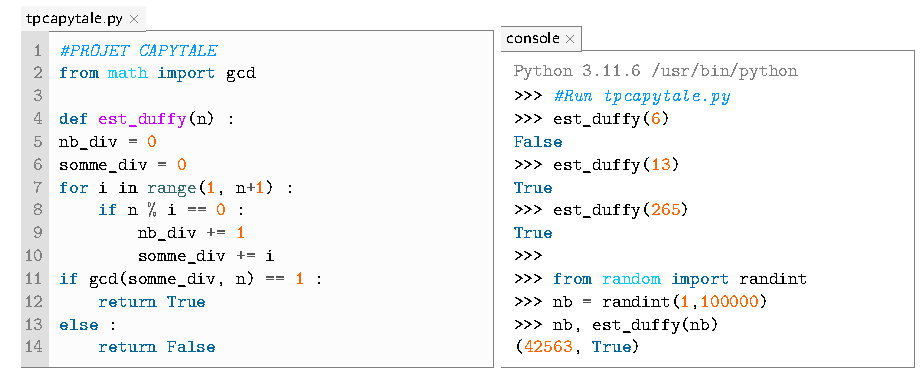
\includegraphics{pitonthonny.pdf}

\newpage

\section{Cartouche Capytale}\label{capytale}

\subsection{Introduction}

\begin{tipblock}
L'idée est d'obtenir des \textsf{cartouches} tels que \textsf{Capytale} les présente, pour partager un code afin d'accéder à une activité \textsf{Python}.
\end{tipblock}

\subsection{Commandes}

\begin{PresCodeTexPL}{listing only}
\CartoucheCapytale(*)[options]{code capytale}
\end{PresCodeTexPL}

\begin{cautionblock}
Peu d'options pour ces commandes :

\begin{itemize}
	\item la version \textit{étoilée} qui permet de  passer de la police \Cle{sffamily} à la police \Cle{ttfamily}, et donc dépendante des fontes du document ;
	\item le deuxième, \textit{optionnel}, permet de rajouter des caractères après le code (comme un \textsf{espace}) ;
	
	\hfill{}défaut \Cle{vide}
	\item le troisième, \textit{obligatoire}, est le \textsf{code capytale} à afficher.
\end{itemize}
\vspace*{-\baselineskip}\leavevmode
\end{cautionblock}

\begin{PresCodeTexPL}{listing only}
\CartoucheCapytale{abcd-12345}           %lien simple, en sf

\CartoucheCapytale[~]{abcd-12345}        %lien avec ~ à la fin, en sf

\CartoucheCapytale*{abcd-12345}          %lien simple, en tt

\CartoucheCapytale*[~]{abcd-12345}       %lien avec ~ à la fin, en tt
\end{PresCodeTexPL}

\begin{PresCodeSortiePL}{text only}
\CartoucheCapytale{abcd-12345}

\CartoucheCapytale[~]{abcd-12345}

\CartoucheCapytale*{abcd-12345}

\CartoucheCapytale*[~]{abcd-12345}
\end{PresCodeSortiePL}

\begin{noteblock}
Le \textsf{cartouche} peut être \og cliquable \fg{} grâce à \ctex{href}.
\end{noteblock}

\begin{PresCodeTexPL}{listing only}
\usepackage{hyperref}
\urlstyle{same}
...
\href{https://capytale2.ac-paris.fr/web/c/abcd-12345}{\CartoucheCapytale{abcd-12345}}
\end{PresCodeTexPL}

\begin{PresCodeSortiePL}{text only}
\href{https://capytale2.ac-paris.fr/web/c/abcd-12345}{\CartoucheCapytale{abcd-12345}}
\end{PresCodeSortiePL}

\newpage

\section{Présentation de code \LaTeX}\label{prescode}

\subsection{Introduction}

\begin{tipblock}
\cmaj{2.0.6} L'idée est de proposer un environnement pour présenter du code \LaTeX. Ce n'est pas forcément lié à l'enseignement en Lycée mais pourquoi pas !

\smallskip

Il s'agir d'un environnement créé en \ctex{tcolorbox}, et utilisant la présentation \textit{basique} de code via \ctex{listings}.
\end{tipblock}

\subsection{Commandes}

\begin{PresCodeTexPL}{listing only}
\begin{PresentationCode}[Couleur]{options tcbox}
...
\end{PresentationCode}
\end{PresCodeTexPL}

\begin{cautionblock}
Peu de personnalisations pour ces commandes :

\begin{itemize}
	\item le premier argument, \textit{optionnel}, permet de préciser la \textit{couleur} de la présentation ;\hfill{}défaut \Cle{CouleurVertForet}
	\item le second, \textit{obligatoire}, correspond aux éventuelles options liées à la \ctex{tcolorbox}.
\end{itemize}
\vspace*{-\baselineskip}\leavevmode
\end{cautionblock}

\begin{noteblock}
Il est à noter que, même dans le cas d'option vide pour la \ctex{tcolorbox}, les \ctex{\{\}} sont nécessaires.

\smallskip

On peut par exemple utiliser l'option \Cle{listing only} pour ne présenter \textit{que} le code source.
\end{noteblock}

\begin{PresCodePL}{}
\begin{PresentationCode}{}
\xdef\ValAleaA{\fpeval{randint(1,100)}}
\xdef\ValAleaB{\fpeval{randint(1,100)}}

Avec $A=\ValAleaA$ et $B=\ValAleaB$, on a $A\times B=\inteval{\ValAleaA * \ValAleaB}$.
\end{PresentationCode}

\begin{PresentationCode}[blue]{}
On peut faire beaucoup de choses avec \LaTeX{} !
\end{PresentationCode}
\end{PresCodePL}
